\setcounter{chapter}{6}

\chapter{常微分方程}

\section{概念与应用}

\subsection{微分方程模型}

{\bf 例:}物体从一定高度开始自由下落,已知其受到的空气阻力与其速度成正比,
求其运动满足的方程。

$$a=g-vk,\quad v'=g-vk,\quad S''=g-S'k$$

{\bf 例}(鱼雷的运动轨迹)
某战舰发现其正东方向1海里处有一艘敌舰以速度$v$向正北方向行驶,于是向其发射鱼雷。
假设鱼雷的速度为$5v$,且其运动方向始终指向敌舰。试给出鱼雷运动轨迹的数学模型。

$$
	\left\{\begin{array}{l}
		5(1-x)y''=\sqrt{1+(y')^2},\;0<x<1,\\
		y(0)=0,\;y'(0)=0.
	\end{array}\right.
$$

{\bf 例}(捕食者-食饵(Predator-Prey)模型)——Lotka-Volterra Equations
$$
	\left\{\begin{array}{l}
		\df{\d x}{\d t}=ax-bxy\\
		\df{\d y}{\d t}=-cy+dxy
	\end{array}\right.
$$

{\bf 例}(疾病传染问题)总人数$N$,已感染$I$,感染率$\gamma$,
治愈率$\lambda$

$$\df{\d I}{\d t}=\gamma (N-I)-\lambda I$$

相对于一般形式的方程,微分方程能够更好地刻画变量、自变量及其相对变化率之间的关系

\subsection{微分方程的有关概念}

{\bf 微分方程:}包含函数、自变量及其相关的微分项的关系式(e.g. 等式)
\ps{同济:表示未知函数、未知函数的导数与自变量之间关系的方程}

{\bf 常微分方程:} 
  $$x''(t)=a,\quad  \df{y''}{(1+y')^{3/2}}=L,\quad 
  L\df{\d i}{\d t}+Ri=E(t)$$ 
  
{\bf 偏微分方程:} 
  $$\df{\p^2U}{\p x^2}+\df{\p^2U}{\p y^2}+\df{\p^2U}{\p z^2}=0,\quad 
  \df{\p^2z}{\p x\p y}=0$$

{\bf ($n$阶)常微分方程:}
$$f(x,y,y',y'',\ldots,y^{(n)})=0$$

\begin{enumerate}[(1)]
  \setlength{\itemindent}{1cm}
  \item {\bf 解:} 使以上方程得到满足的函数$y=\varphi(x)$ 
  \item {\bf 通解:}含有$n$个相互独立的任意常数的解  
  \item {\bf 特解:}不存在任何未确定常数的解 
  \begin{itemize}
    \item $n$阶方程的通解需包含$n$个相互独立的任意常数
    \item 通解有时候不代表全部的解
    \item 通过定解条件来确定响应的特解
    \item 微分方程的通解表达式不唯一
  \end{itemize} 
  \item {\bf 初值问题/Cauchy问题:}
  $$
  \left\{\begin{array}{l}
  	f(x,y,y',y'',\ldots,y^{(n)})=0\\
  	\quad{y^{(n-1)}(x_{n-1})=y_{n-1}}\\
  	\quad{\ldots\ldots\ldots\ldots}\\
  	\quad{y'(x_1)=y_1}\\
  	\quad{y(x_0)=y_0}
  \end{array}\right.
  $$
  \item {\bf 积分曲线:}微分方程的解所对应的曲线
\end{enumerate}

{\bf 例:}$y''+y=0$的两个特解$y=\sin x,\;y=\cos x$,其通解是:(D)
\begin{enumerate}[(A)]
  \setlength{\itemindent}{1cm}
  \item $y=C_1\sin x$
  \item $y=C_1\sin x+C_2\sin x$
  \item $y=C_1\sin x+\cos(C_2x)$
  \item $y=C_1\sin x-C_2\cos x$
\end{enumerate}
求满足$y(0)=0,\;y'(\pi)=1$的(特)解。

\section{一阶微分方程的解法}

绝大多数微分方程的解都是无法解析求得的!\ps{更多需要依赖数值方法}

{\bf 一阶微分方程:}
$$f(x,y,y')=0$$ 
\begin{itemize}
  \item 可分离变量的方程 
  \item 齐次方程 
  \item 一阶线性微分方程 
  \item 一些特殊形式的微分方程
\end{itemize}

\subsection{可分离变量的方程}

$${\df{\d y}{\d x}=f(x)g(y)}$$ 
{\bf 解法:}
$$\df{\d y}{g(y)}=f(x)\d x,\;(g(y)\ne 0)$$ 
上式两边分别关于$x,y$求不定积分,得:
$$\dint\df{\d y}{g(y)}=\dint f(x)\d x+C$$ 
整理化简后既得方程的解。

{\bf 例:}
\begin{enumerate}[(1)]
  \setlength{\itemindent}{1cm}
  \item $y'=xy$\ps{分离变量时,对分母为零的情况要单独讨论!!}
  \item $\df{\d y}{\d x}=3\sin x\cos^2 y$
  \item $(e^{x+y}-e^x)\d x+(e^{x+y}+e^y)\d y=0$\hfill $(e^x+1)(e^y-1)=C$
\end{enumerate}

{\bf 例:}已知曲线$C$上任一点$P(x,y)$处的法线与$x$轴交点为$Q$,且线段$PQ$被$y$轴平分,
求曲线$C$所满足的方程。

$$yy'+2x=0$$

\subsection{齐次方程}

$${\df{\d y}{\d x}=\varphi\left(\df yx\right)}$$

{\bf 例如:}
$$x^2y'=y^2,\quad y'=\df{y^2-x^2}{xy}$$ 
{\bf 解法:}令$z=y/x$, 则
$$\df{\d y}{\d x}=z+x\df{\d z}{\d x}\quad\Rightarrow\quad
x\df{\d z}{\d x}+z=\varphi(z)$$

{\bf 例:}
\begin{enumerate}[(1)]
  \setlength{\itemindent}{1cm}
  \item $y'=\df{x-y}{x+y}$\hfill $y^2+2xy-x^2=Cx^2e^{-x^2}$
  \item $(3y^2+x^2)\d y+2xy\d x=0$\hfill P408-例3(书上第一个加号是减号!)
\end{enumerate}

{\bf P408-例4:}$y'=\df{2x-5y+3}{2x+4y-6}$

{\bf 思路:}令$x=X+h,y=Y+k$,带入原方程,解出$h,k$的值,使新的方程
化为齐次方程。

$$x=X+1,\;y=Y+1$$

\subsection{一阶线性微分方程}

{\bf ($n$阶)线性微分方程:}
$$y^{(n)}+a_{n-1}(x)y^{(n-1)}+\ldots+a_1(x)y'+a_0(x)y=f(x)$$

{\bf 一阶齐次线性微分方程:}
$$y'+p(x)y=0$$
通解:$y=Ce^{-\int p(x)dx}$

{\bf 一阶(非齐次)线性微分方程:}
$$y'+p(x)y=q(x)$$

{\bf 常数变异法:}令齐次方程通解中的$C=C(x)$,代入非齐次方程,得
$$\left(C(x)e^{-\int p(x)dx}\right)'+p(x)C(x)e^{-\int
 p(x)dx}=q(x)$$
即
$$C'(x)e^{-\int p(x)dx}=q(x)$$
从而
$$C(x)=\dint q(x)e^{\int p(x)dx}dx+C$$ 

{\bf 一阶非齐次线性微分方程的通解:}
$$y=Ce^{-\int p(x)dx}+e^{-\int p(x)dx}\dint q(x)e^{\int p(x)dx}dx$$

\begin{shaded}
{\bf 常数变异法的构造思路}

$$\left(ye^{\int p(x)\d x}\right)'_x=e^{\int p(x)\d x}[y'+p(x)y]
=q(x)e^{\int p(x)\d x}$$

关于{\it 积分因子}的有关解释参加{\bf 辅导书(下)-P228}
\end{shaded}

{\bf 例:}$y'=\df1{x+y}$\hfill 习题7.2-4(1)

\subsection{Bernoulli方程}

$$y'+P(x)y=Q(x)y^n\;(n\ne 0,1)$$ 
方程两边同时除以$y^n$,得
$$y^{-n}y'+P(x)y^{1-n}=Q(x)$$ 
令$z=y^{1-n}$,则
$$z'+(1-n)P(x)z=(1-n)Q(x)$$

{\bf 例:}
\begin{enumerate}[(1)]
  \setlength{\itemindent}{1cm}
  \item $y'-\df{y}{2x}=\df{x^2}{2y}$
  \item $y'=\df{x}{x^2+y^2}$\hfill$x^2+y^2+y+\df12=Ce^{2y}$
  \item $y'=xy(3+y)$\hfill$\left(Ce^{-\frac32x^2}-\df13\right)y=1$
  \item $y'=\df{x^3+y^3}{3xy^2}$\hfill$y^3=\df{x^3}2+Cx$
\end{enumerate}

\subsection{Clairaut方程}
$$y=xy'+f(y')$$
两边对$x$求导,
$$0=(x+f'(y'))y''$$

{\bf 例:}$y=xy'\pm\sqrt{-y'}$\hfill 习题7.3-3:$y=Cx\pm2\sqrt{-C},\,xy=1$

\bigskip

{\bf 课堂思考题:}
\begin{enumerate}[(1)]
  \setlength{\itemindent}{1cm}
  \item $y'=(x+y)^2$\hfill 令:$z=x+y$
  \item $(\sin x+y)\d x+(x+\cos y)\d y=0$\hfill 微分运算
  \item $x\ln x\d y+(y-\ln x)\d x=0$\hfill 令:$t=\ln x$
\end{enumerate}

\section{特殊二阶方程的解法}

\subsection{$y''=f(x,y')$型微分方程}

{\bf P418-例2:}$xy''-y'=0$\hfill $y=\df12C_1x^2+C_2,\;(C_1,C_2\in\mathbb{R})$

{\bf 解法:}令$y'=p(x)$,将原方程化为关于$p$和$x$的微分方程$\df{\d p}{\d x}=f(x,p)$

{\bf 例:}$y'y'''=3(y'')^2$\hfill $x=C_1y+C_2y+C_3$

\subsection{$y''=f(y,y')$型微分方程}

{\bf P418-例3:}$yy''+(y')^2=0$\hfill $y^2=C_1x+C_2,\;(C_1,C_2\in\mathbb{R})$

{\bf 解法:}令$y'_x=p(y)$,则$\df{\d^2y}{\d x^2}=p\df{\d p}{\d y}$,
原方程化为关于$p$和$y$的微分方程$$\df{\d p}{\d y}=\df{f(y,p)}{p}$$

{\bf 思考:}
\begin{enumerate}[(1)]
  \setlength{\itemindent}{1cm}
  \item 如何求解形如$y'''=f(x,y'')=0$或$y'''=f(x,y'')=0$的微分方程?
  \item 以上方法还可以如何加以推广?\hfill$y^{(n)}=f(x,y^{(n-1)}),
  \,y^{(n)}=f(y,y^{(n-1)})$
  \item 总结归纳一下我们还可以求解哪些不低于二阶的微分方程?\\
  $y''=f(x),\;y''=f(y),\;y''=f(x,y'),\;y''=f(y,y'),
  \;y''=f(y'),\;y'''=f(y',y'')$,但是$y''=f(x,y)$呢?
\end{enumerate}

\section{二阶线性微分方程}

{\bf $n$阶线性微分方程:}
$$y^{(n)}+a_{n-1}(x)y^{(n-1)}+\ldots+a_1(x)y'+a_0(x)y=f(x)$$

\begin{itemize}
  \setlength{\itemindent}{1cm}
  \item {\bf 二阶齐次线性微分方程}
  $${y''+p(x)y'+q(x)y=0}$$
  \item {\bf 二阶非齐次线性微分方程}
  $${y''+p(x)y'+q(x)y=f(x)}$$
\end{itemize}

\subsection{二阶线性微分方程解的结构}

{\bf 定理7.4.1-7.4.2:}
若$y_1(x),y_2(x)$为二阶齐次线性微分方程
$$y''+p(x)y'+q(x)y=0$$
的两个解,则 
\begin{enumerate}[(1)]
  \setlength{\itemindent}{1cm}
  \item 线性组合${y=C_1y_1+C_2y_2}$($C_1,C_2$为任意常数)仍为该方程的解; 
  \item 若$y_1,y_2${\underline{线性无关}},则以上线性组合即为该方程的通解。
\end{enumerate}

{\bf 问:}什么叫做两个函数线性无关?(比值不为常数!)

{\bf 辅导书(下)-P241-例10-14:}求以$x$和$e^x$为特解的二阶齐次线性微分方程。

$$(x-1)y''-xy'+y=0$$

{\bf 定理7.4.3:}
若$y^*$是二阶非齐次线性微分方程
$$y''+p(x)y'+q(x)y=f(x)\eqno{(1)}$$
的一个特解,$Y$是对应齐次方程的通解,则该方程的通解的通解为$y=Y+y^*$。

{\bf 例:}已知微分方程$(1)$的三个解:$y_1=x,y_2=e^x,y_3=e^{2x}$,
求其满足初始条件$y(0)=1,y'(0)=3$的特解。

{\bf 定理}(叠加原理)\hfill{习题7.4-11}

若$y_i(i=1,2,\ldots,m)$分别为方程
$$y''+p(x)y'+g(x)y=f_i(x),\;i=1,2,\ldots,m$$
的解,则$\sum\limits_{i=1}^my_i$为
$$y''+p(x)y'+g(x)y=\sum\limits_{i=1}^mf_i(x)$$
的解。

{\bf 注:}叠加原理对于高阶的线性非齐次微分方程仍然成立!

\subsection{二阶线性微分方程的解法}

\subsubsection{降阶法求二阶其次线性微分方程的特解}

{\bf 问题:}已知$y_1(x)$为齐次方程$y''+p(x)y'+q(x)y=0$的一个特解$y_1$,
如何求得另一个与之线性无关的特解$y_2$?

{\bf Liouville公式:}设$y_2=uy_1$,其中$u=u(x)$待定\ps{这样假设
需要满足什么特殊的条件吗?}。则
$$u{(y''_1+py'_1+qy_1)}+u'(2y'_1+py_1)+y_1u''=0,$$ 
即$u'(2y'_1+py_1)+y_1u''=0$, 由此可解得
$${u(x)=\dint\df{e^{-\int p(x)dx}}{y_1^2}dx}$$

{\bf 思考:}形如$y=uy_1$的变换的好处是什么?能够推广到更高阶的情形吗?

答:将方程最低阶项的系数化为$0$。对于更高阶的齐次线性方程,该变化同样有效!

{\bf P424-例2:}已知$y=e^x$为方程
$$y''+\df{x}{1-x}y'-\df{1}{1-x}y=0$$
的解,求该方程的通解。\hfill $y=C_1x+C_2e^x$

{\bf 辅导书(下)-P242-例10-16(1):}$xy''-y'-(x-1)y=0$
$$y_1=e^x,\;y=C_1e^x+C_2(2x+1)e^{-x}$$

\subsubsection{二阶常系数齐次线性微分方程的通解}

$$y''+py'+qy=0\;(p,q\in\mathbb{R}\mbox{为常数})$$

{\bf 特征方程(根)法:}设$y=e^{rx}$为方程的解,则
$$e^{rx}(r^2+pr+q)=0$$ 
即:$r^2+pr+q=0$ 。显然,若$r$为该{\bf 特征方程}的根,则
$y=e^{rx}$为原方程的解。

{\bf P426-表7.4.1}(死记!)
记$\Delta=p^2-4q$, 则:
\begin{center}
	\begin{tabular}{c|c|c|c}
		\hline
		{$\Delta$} & {$r$} & {特解} & {通解} \\ \hline 
		$\Delta>0$ & \begin{tabular}{cc}相异实根 \\ $r_1,r_2$\end{tabular} &
		$\begin{array}{ll}y_1=e^{r_1x}\\ y_2=e^{r_2x}\end{array}$ &
		{$C_1e^{r_1x}+C_2e^{r_2x}$}\\ \hline 
		$\Delta=0$ & 二重实根$r$ &
		$\begin{array}{ll}y_1=e^{rx}\\ y_2=xe^{rx}\end{array}$ &
		{$(C_1+xC_2)e^{rx}$}\\ \hline 
		$\Delta<0$ & \begin{tabular}{cc}共轭复根\\ $\alpha\pm i\beta$\end{tabular} &
		$\begin{array}{ll}y_1=e^{\alpha x}\cos\beta x\\ y_2=e^{\alpha
		x}\sin\beta x\end{array}$ & 
		{$\begin{array}{ll}e^{\alpha x}(C_1\cos\beta x +C_2\sin\beta
		x)\end{array}$}\\ \hline
	\end{tabular}
\end{center}

注:$\Delta=0$时,$y_1=e^{rx}$,由Liouville公式
$$y_2=y_1\dint\df{e^{\int p\d x}}{y_1^2}\d x
=e^{rx}\dint e^{-(p+2r)x}\d x=e^{rx}\dint\d x=xe^{rx}$$

{\bf P426-例3-5}(自行阅读)
\begin{enumerate}[(1)]
  \setlength{\itemindent}{1cm}
  \item $y''-y'-2y=0$
  \item $\df{\d^2s}{\d t^2}+2\df{\d s}{\d t}+s=0$
  \item $y''-2y'+5y=0$
\end{enumerate}

\subsubsection{用常数变异法求二阶非齐次线性微分方程}

\begin{shaded}
{\bf 辅导书(下)-P231:}
设$y_1,y_2$是对应二阶齐次线性微分方程的线性无关的解,令

$$
\left\{\begin{array}{l}
y_1C'_1+y_2C'_2=0\\
y_1'C_1'+y'_2C'_2=f(x)
\end{array}\right.
$$
解出$C_1(x)$和$C_2(x)$,则$y^*=C_1(x)y_1+C_2(x)y_2$为非齐次方程的一个特解。
\end{shaded}

{\it 常数变异法在二阶常微分方程中的应用,陈文胜,2001}

考虑
$$y''+py'+qy=f(x)$$
特征方程
$$r^2+pr+q=0$$
根据其根为实数或复数分别考虑如下:

(1)若$r\in\mathbb{R}$,则$y=Ce^{rx}$为对应齐次方程的解,从而设特解
$y=C(x)e^{rx}$,于是
$$C''+(2r+p)C'=e^{-rx}f(x)$$
$$C(x)=\dint\left[e^{-(2r+p)x}\dint e^{(r+p)x}f(x)\d x\right]\d x$$

{\bf 例:}$y''+y'-2y=\sin x$

设$y=C(x)e^x$,则
$$C''+3C'=e^{-x}\sin x$$
解得
$$C(x)=-\df1{10}(3\sin x+\cos x)e^{-x}+C_1e^{-3x}+C_2$$

{\bf 例:}$y''+4y'+4y=e^x$

通解$y=\df19e^x+C_1xe^{-2x}+C_2e^{-2x}$

(2)若$r=\alpha+i\beta\in\mathbb{C}$,则$y=Ce^{\alpha x}\sin\beta x$
为齐次方程的解,从而设特解$y=C(x)e^{\alpha x}\sin\beta x$,类似地可得
$$C(x)=\dint\left(\df{e^{-(p+2\alpha)x}\dint f(x)
e^{(p+\alpha)x}\sin\beta x\d x}{\sin^2\beta x}\right)\d x$$

{\bf 例:}$y''+y=\df1{\cos x}$

$$y=\sin x\dint\df{\dint\tan x\d x}{\sin^2 x}\d x
=\sin x(\ln|\cos x|+C_1\cos x+(x+C_2)\sin x)$$

{\bf 思考:}以上方法能否推广到非常系数的情形?

\subsubsection{(部分)二阶常系数非齐次线性方程的解法}

关键是求得该方程的一个特解!

{\bf 【情形一】:}$f(x)=e^{\lambda x}P_m(x)$,其中$P_m(x)$为$m$阶多项式,
$\lambda$为常数

{\bf 解法:}设方程的特解为
$$y^*=x^ke^{\lambda x}(a_0+a_1x+\ldots+a_mx^m),$$
其中$k=0,1,2$分别对应与$\lambda$不是特征方程的根、
是特征方程的重根和单根的情况

% \newpage

{\bf P427-例6:}$y''-2y'-3y=e^{3x}(1+x^2)$

{\bf 教材上的解法:}
设原方程有特解$y^*=e^{3x}x(a_0+a_1x+a_2x^2)$,代回原方程利用待定系数法解得
$a_0=\df9{32},a_1=-\df1{16},a_2=\df1{12}$,
故该方程的通解为
$$y=C_1e^{-x}+C_2e^{3x}+e^{3x}x\left(\df9{32}-\df{x}{16}+\df1{12}x^2\right)$$

\begin{shaded}
	{\bf 用常数变异法求解:}
	显然,该方程对应的齐次方程的通解为$C_1e^{-x}+C_2e^{3x},(C_1,C_2\in\mathbb{R})$。
	设$y^*=C(x)e^{3x}$为原方程的一个特解,带入方程化简可得
	$$C''+4C'=1+x^2\eqno{(E1)},$$
	令$C'=w(x)$,方程(E1)化为$w'+4w=1+x^2$,利用一阶线性微分方程的常数变易法可解得
	$C'=w=\df9{32}-\df18x+\df14x^2+C_3$,不妨令$C_3=0$,进而可得
	$$C(x)=\df9{32}x-\df1{16}x^2+\df1{12}x^3+C_4.$$
	不妨令$C_4=0$,从而可得原方程的通解为
	$$y=C_1e^{-x}+C_2e^{3x}+e^{3x}x\left(\df9{32}-\df{x}{16}+\df1{12}x^2\right),
	(C_1,C_2\in\mathbb{R}).$$
	
	{\bf 注:}{\it 以上两种解法都存在很大的计算量,但是相对而言,使用常数变易法解题的思路更为
	直观清晰,便于随时检查验算阶段性的计算结果,推荐使用。}
\end{shaded}

% \newpage

{\bf 例}(习题7.4-11(2))$y''-6y'+9y=e^{3x}+9$
$$y=C_1e^{3x}+C_2xe^3x+\df12x^2e^{3x}+1$$

{\bf 【情形二】:}$f(x)=e^{\alpha x}[P_m(x)\cos\beta x+P_l(x)\sin\beta x]$,
其中$P_m(x),P_l(x)$分别为$m,l$阶多项式,$\beta\ne 0$

{\bf 解法:}设方程的特解为
$$y^*=x^ke^{\alpha x}[R^{(1)}_n(x)\cos\beta x+R^{(2)}_n(x)\sin\beta x]$$ 
其中:$n=\max\{m,l\}$,$R^{(1)}_n(x),R^{(2)}_n(x)$均为次数不超过$n$的多项式;
若$\alpha+i\beta$是特征方程的根,取$k=1$,否则取$k=0$。 

{\bf P428-例7:}$y''+4y=\cos 2x$

设$y^*=x(A\cos2x+B\sin2x)$,通解
$$y=C_1\cos2x+C_2\sin2x+\df x4\sin2x$$

\subsubsection{Eular方程}

$$x^2y''+pxy'+qy=f(x)\;(p,q\in\mathbb{R}\mbox{为常数})$$

{\bf 解:}令$x=e^t$,则
$$y'_x=\df1xy'_t,\;y''_{xx}=\df1{x^2}(y''_{tt}-y'_t),$$
即
$$x^2y''_{xx}=y''_{tt}-y'_t,\;xy'_x=y'_t,$$
原方程可化为二阶常系数线性微分方程
$$y''_{tt}+(p-1)y'_t+qy=f(e^t)$$

{\bf P432-例9:}$x^2y''+xy'-y=0$

$$y''_tt-y=0,\quad y=\df{C_1}x+C_2x$$

{\bf 思考:}以上解法对于我们求解高阶方程有何启示?\hfill{\bf 辅导书(下)-P230}

事实上,$x^3y'''_{xxx}=\df1{x^3}(y'''_{ttt}-3y''_{tt}+2y'_t)$,故
以上的方法可以推广到三阶,特别是$f(x)=0$的情形,例如:
$$x^3y'''+px^2y''+qxy'+ry=0$$

那么,还可以进一步推广吗?请课后自行推理!

\section{小结与习题课}

\subsection{本章小结}

\begin{enumerate}[1]
%   \setlength{\itemindent}{1cm}
  \item 基本概念
  \begin{enumerate}[(1)]
    \item 通解、特解、初值问题
    \item {\it 积分曲线、线素场}*
  \end{enumerate}
  \item 一阶微分方程
  \begin{enumerate}[(1)]
    \item 可分离变量的方程\dotfill$\df{\d y}{g(y)}=f(x)\d x$
    或$g(y)=0$
    \item 一阶线性微分方程\dotfill 常数变易法
    \item 齐次方程\dotfill$z=\df yx$
    \item Bernoulli方程\dotfill$z=y^{1-n},n\ne0,1$
  \end{enumerate}
  \item 两类可降阶的方程(情形)
  \begin{enumerate}[(1)]
    \item $y''=f(x,y')$\dotfill$y'=p(x)$;可推广到$y^{(n)}=f(x,y^{(n-1)})$
    \item $y''=f(y,y')$\dotfill$y'=p(y)$;不能直接推广到$y^{(n)}=f(y,y^{(n-1)})$
  \end{enumerate}
  \item 二阶线性微分方程
  \begin{enumerate}[(1)]
    \item 解的结构(对于高阶的线性微分方程仍然成立)
    \begin{itemize}
      \item 若齐次方程的有线性无关的特解$y_1,y_2$,则通解为:
      $$Y=C_1y_1+C_2y_2,\;(C_1,C_2\in\mathbb{R})$$
      \item 若非齐次方程有特解$y^*$,则通解为$Y+y^*$
      \item {\it 叠加原理*}
    \end{itemize}
    \item $\bm{y=uy_1}$:已知齐次方程的特解$y_1$,求其他特解
    \begin{itemize}
      \item 齐次方程\dotfill Liouville公式
      \item 非齐次方程\dotfill 常数变易法的二阶推广
    \end{itemize}
    \item 常系数齐次线性微分方程的通解\dotfill 特征根法;可以推广到高阶的常系数线性微分方程
    \item Eular方程:\dotfill $x=e^t$,原方程化为常系数线性微分方程
  \end{enumerate}
\end{enumerate}

\subsection{问题讨论}

{\bf 例:}判定分析
\begin{enumerate}[(1)]
  \setlength{\itemindent}{1cm}
  \item 以下推导是否正确? 
	$$xy'=y\quad \Rightarrow\quad y=0\;\mbox{或}\;\df{\d y}{y}=\df{\d x}{x}$$
	 $$\Rightarrow\quad y=0\;\mbox{或}\;\ln |y|=\ln
	|x|+C_1\;(C_1\in\mathbb{R})$$
	 
	故方程通解为:
	$$y=Cx\;\quad (C\in\mathbb{R})$$
	 	
	{\bf 答:}正确!
  \item  已知$n$阶线性微分方程的$n$个解,能否写出这个微分方程及其通解? 
	
  {\bf 答:}不一定。 除非{这$n$个解恰为$n$阶齐次线性微分方程的线性无关的特解。} 
  \item 适当确定微分方程通解中的参数值,可以得到其任意的特解? 
	
  {\bf 答:}错!反例:$xy'=y^2$。
  \item $y_1=(x-1)^2$和$y_2=(x+1)^2$ 都是方程
	$$(x-1)^2y''-2xy'+2y=0,$$
	和
	$$2yy''-(y')^2=0$$
	的解。 但二者的线性组合
	$$y=c_1(x-1)^2+c_2(x+1)^2,\;(c_1,c_2\in\mathbb{R})$$
	 却仅能满足前一个方程, 为什么?
  
  {\bf 答:}第二个方程不是齐次线性方程!
  \item 求以$(x+C)^2+y^2=1$为通解的微分方程。
  {\bf 答:}$(y')^2=\df1{y^2}-1$。
\end{enumerate}

\subsection{方程求解}

{\bf 例}(合理利用变换和技巧求解微分方程)

\hspace{-1ex}{\bf 【上下颠倒】}
\begin{enumerate}[(1)]
  \setlength{\itemindent}{1cm}
  \item $y'=\df{1}{2x-y^2}$ \dotfill{“上下颠倒”},$x=\df12y(y+1)+\df14+Ce^{2y}$
  \item $y'=\df{x}{x^2-y^2}$\dotfill{“上下颠倒”化为Bernoulli方程}\\
  {\bf 【齐次方程】}
  \item $xy'=\sqrt{x^2-y^2}+y$ \dotfill{齐次方程},$y=x\sin(\ln|x|+C)$
  \item $y'=\df{3x^2+y^2-6x+3}{2xy-2y}$
  \dotfill{消去低次项变齐次方程},$3(x-1)^2-y^2=C(x-1)$\\
  {\bf 【其他变量替换】}
  \item $xy'+y=2\sqrt{xy}$\dotfill{ 令$u=xy$},$\sqrt{xy}=x+C$
  \item $xy'+y=y(\ln x+\ln y) $ \dotfill{令$z=\ln x, w=\ln y$或$z=xy$},$xy=Ce^x$
  \item $xy'\ln x+y=ax(\ln x+1)$\dotfill{ 一阶线性方程},$y=\df12\ln x+\df C{\ln x}+1$
  \item $y'=\df{y}{2(\ln y-x)}$\dotfill{ “颠倒”,令$z=\ln y$},$y^2[1-2(\ln y-x)]=C$
  \item $y'+x=\sqrt{x^2+y}$\dotfill{ 令$z=\sqrt{x^2+y}-x$},
  $x^2+y=(x+C)(2\sqrt{x^2+y}-x)$\\
  {\bf 【Bernouli方程】}
  \item $y'-\df{y}{x}=\df{2x}{3y^2}$ \dotfill{Bernouli方程},$y^3=Cx^3-2x^2$
  \item $2x\ln x\d y+y(y^2\ln x-1)\d x=0$\dotfill{令$z=\ln x$,Bernouli方程}\\
  \hfill $\df1{y^2}=\df12\ln x+\df C{\ln x}$\\
  {\bf 【降阶计算】}
  \item $y^{(4)}+y''=0$\dotfill{ 令$p=y''$}
\end{enumerate}

{\bf 例}(全微分方程)
\begin{enumerate}[(1)]
  \setlength{\itemindent}{1cm}
  \item $(e^x+e^{x+y})\d x+(e^y+e^{x+y})\d y=0$
  \item $(3y^2+2xy)\d y+(y^2+5x^4)\d x=0$
  \item $x\d x+y\d y+\df{y\d y-x\d x}{x^2+y^2}=0$
  \item $y\d x+x\d y+\df{x\d y-y\d x}{x^2+y^2}=0$\dotfill$xy+\arctan\df yx=C$ 
\end{enumerate}

\subsection{综合推导}

{\bf 习题7.2-7:}已知$f(x)$在$\mathbb{R}$上有定义,且对任意$x,y$,有
$f(x+y)=f(x)f(y)$,又$f'(0)=2$,求$f(x)$。

{\bf 辅导书(下)-P256-例5:}$f'(0)=2$,
$$f(x+y)=xf(y)+f(x)f(y)+yf(x)-(x-xy+y)$$
$$f'(x)=3f(x)+3x-1,\;f(0)=1\Rightarrow f(x)=e^{3x}-x$$

{\bf 例:}设$F(x)=f(x)g(x)$,且$f'(x)=g(x),\;g'(x)=f(x)$,
$f(0)=0$,$f(x)+g(x)=2e^x$
\begin{enumerate}[(1)]
  \setlength{\itemindent}{1cm}
  \item 求$F(x)$所满足的一阶微分方程;
  \item 求$F(x)$的表达式;
  \item 求$f(x),g(x)$的表达式。
\end{enumerate}

{\bf 例:}求满足$\dint f(x)\d x\dint\df1{f(x)}\d x=1$的所有函数。

$$f'(x)=\pm f'(x),\;f(x)=Ce^{\pm x}$$

{\bf 例:}设$\varphi(x)=e^x-\dint_0^x(x-u)\varphi(u)du,$
其中$\varphi(x)$连续,求其函数表达式。

{\bf 例:}设$\varphi'(x)=e^x+\sqrt x\dint_0^{\sqrt x}\varphi(\sqrt x u)du,$
$\varphi(0)=0$,求$\varphi(x)$。

{\bf 例:}某学生将乘积的导数公式错误地记作$(fg)'=f'g'$,然而在一次求导时居然得到了正确的结果。
目前知道他使用的$f(x)=e^{x^2},(x>1/2)$,问他用到的$g(x)$可能是什么?

$$\left(e^{x^2}g\right)'=\left(e^{x^2}\right)'g'$$
从而$(2x-1)g'=2xg$,解得$g=Ce^x\sqrt{|2x-1|}$

{\bf 辅导书(下)-P257-例8}(2003年考研)
设$y(x)$在$\mathbb{R}$上具有二阶连续导数,$y'\ne 0$,$x=x(y)$
为其反函数。
\begin{enumerate}[(1)]
  \setlength{\itemindent}{1cm}
  \item 试将$x=x(y)$所满足的微分方程
  $$\df{\d^2x}{\d y^2}+(y+\sin x)\left(\df{\d x}{\d y}\right)^3=0$$
  变换为$y=y(x)$所满足的微分方程;\hfill$y''-y=-\sin x$
  \item 求变换后的微分方程满足初始条件$y(0)=0$和$y'(0)=1.5$的解。
\end{enumerate}
设特解$y^*=A\cos x+B\sin x$,解得$A=0,B=1/2$,故通解
$$y=C_1e^x+C_2e^{-x}+\df12\sin x,$$
利用初值条件,得所求特解
$$y=e^x-e^{-x}+\df12\sin x$$

\begin{shaded}
{\bf 用常数变易法:}令$y^*=C(x)e^x$,则$C''+2C'=-e^x\sin x$。令$w=C'$,解得
$w=-\df12e^x(\sin x-\cos x)$,进而$C=\df12\sin xe^{-x}$,从而$y^*=\df12\sin x$
\end{shaded}
		
\subsection{应用题}

{\bf 习题7.2-12:}某湖泊的水量为$V$,每年排入湖内的污水和净水量均为$V/6$,且湖内的总水量不变。
已知1999年底湖内的污染物含量为$5m_0$。为了治理污染,从2000初开始,限定排入
湖中的污水中污染物浓度不得超过$m_0/V$。问至少需要经过多少年,
湖内的污染物含量能够降至$m_0$以下?(注:假设湖水中的污染物浓度时均匀分布的。)

$$m'=\df{m_0}6-\df m3,\quad m=\df{m_0}2(1+9e^{-t/3})$$

$t=6\ln3$年后,达到要求。

{\bf 例:}已知某车间容积$V$,其空气中CO$_2$的密度为$\rho_1$,现以CO$_2$浓度$\rho_2(<<\rho_1)$的
新鲜空气输入,问每分钟应输入多少才能在$T$分钟后使车间中CO$_2$的含量不超过$\rho_0$。
({\bf 注:}假设新注入的空气能够与原有空气立即混合达到均匀,且空气不会被压缩。)

$$C'=\rho_2V_1-C\df{V_1}{V},C(0)=\rho_1V$$

% $t$分钟时的CO$_2$含量
% $$C(t)=54\left[0.08\mathrm{exp}
% \left(-\df{\overline{V}t}{5400}\right)+0.04\right]$$

{\bf 例:}设河边点$O$的正对岸为点$A$,河宽$h$,两岸平行,水流速度恒定为$a$。
一只鸭子从点$A$游向点$O$,游动过程中其始终朝向$O$点。已知鸭子在
静水中的游速为$b(b>a)$,求鸭子的运动轨迹。

以$O$为坐标原点,$A$点坐标为$(0,h)$,则
$$\df{\d x}{\d y}=\df ab\sqrt{\left(\df xy\right)^2+1}-\df xy$$
初值条件$x(h)=0$

{\bf 习题7.4-14:}一根挂在钉子上的链条,最初两端距离钉子分别为$8$m和$12$m,如不计钉子
对链条产生的摩擦力,求链条从钉子上完全滑落所需的时间。

设$x$为较长一端端点据钉子的距离
$$\left\{\begin{array}{l}
	x''-\df g{10}x=-g\\
	x(0)=12\\
	x'(0)=0
\end{array}\right.$$

{\bf 习题7.3-3:}求第一象限中的一条曲线,使其上每一点处的切线与两坐标轴所围三角形的
面积等于$2$。

[hint]:由题意
$$\df12\left(x-\df y{y'}\right)(y-xy')=2,$$
整理得
$$y=xy'\pm2\sqrt{-y'}.$$
解之可得
$$y=Cx\pm2\sqrt{-C}\mbox{或}xy=1$$

\begin{shaded}

{\bf 例}(Einstein的宇宙膨胀模型)假定宇宙是一个球体(半径$R(t)$),$t$表示时间,则
$$R''=-\df{GM_0}{R^2}$$
其中$G$为宇宙引力常数,$M_0$为宇宙质量。通过分析该方程可以得到关于宇宙膨胀的一些有趣的知识。

方程两端乘以$R'$可得
$$R''R'=-\df{GM_0}{R^2}R'$$
也即
$$[(R')^2]'=2GM_0\left(\df1R\right)'$$
积分可得
$$(R')^2=\df{2GM_0}R+C$$
其中$C$是和宇宙膨胀初始速度有关的常数。

下面利用上式($R'$和$R$之间的关系)确定宇宙半径是如何随时间变化的。

(1)$C>0$,此时
$$R'=\pm\sqrt{\df{2GM_0}R+C},$$
观测表明当前宇宙是膨胀的,故$R'>0$。由此可见,随着$R$越来越大,其膨胀的速度将越来越小,最终趋于
常数$\sqrt C$

(2)$-\df{2GM_0}R<C<0$,记$C=-K$,则
$$R'=\pm\sqrt{\df{2GM_0}R-K},$$
假定在某个时刻$t_0$宇宙是膨胀的,则$R'=\sqrt{\df{2GM_0}R-K}$,并且此时$\df{2GM_0}R>K$,
从而可知,当宇宙半径增加至$\df{2GM_0}R=K$时,宇宙将停止膨胀。此后,如果在某个时刻,有某种因素
引起宇宙收缩,则$R$满足
$$R'=-\sqrt{\df{2GM_0}R-K},$$
当$R$越来越小时,$\sqrt{\df{2GM_0}R-K}$越来越大,最终趋于正无穷。在此过程中,宇宙收缩的速度将
越来越快,最终发生“大坍缩”。

(3)$C=0$。假定在某个时刻宇宙是膨胀的,则
$$R'=\sqrt{\df{2GM_0}R},$$
解之可得
$$R^{\frac32}=\df32\sqrt{2GM_0}t+C_1$$
称为“平直宇宙模型”(flat universe model)

{\bf 注:}以上模型仅仅是当时科学界的一种看法,近年来,科学界又对宇宙膨胀提出了一些新的解释,比如
暗能量解释等。

\end{shaded}

\newpage

\section*{课后作业}

{\bf 【基本题】}

\begin{itemize}
  \setlength{\itemindent}{1cm}
  \item 习题7.1:7
  \item 习题7.2:3,4(2,3,5,6),5,6
  \item 习题7.3:1,2(1,3,5)
  \item 习题7.4:6
\end{itemize}

{\bf 【上交题】}

\begin{itemize}
  \setlength{\itemindent}{1cm}
  \item 习题7.1:8,10-14
  \item 习题7.2:7,8,10
  \item 习题7.3:4,7
  \item 习题7.4:12,13,14(1)
\end{itemize}


{\bf 【思考题】}

\begin{itemize}
  \setlength{\itemindent}{1cm}
  \item 习题7.2:12
  \item 习题7.3:3,5
  \item 习题7.4:8,9,11,13,15,16
\end{itemize}

\newpage

\begin{center}
	{\Large\bf 补充习题参考解答:}
\end{center}


{\it 注:以下题目的编号和顺序可能与作业有所不同,请留意!欢迎纠错:)}

(1)$y'=\df1{2x-y^2}$

{\bf 解:}原方程即为
$$\df{\d x}{\d y}-2x=-y^2,$$
由一阶非齐次线性微分方程的常数变易法,解得
$$x=\df12y(y+1)+\df14+Ce^{2x},(C\in\mathbb{R})$$

(2)$y'=\df{x}{x^2-y^2}$

{\bf 解:}原方程即为
$$\df{\d x}{\d y}-x=-\df{y^2}x,$$
该方程为Bernoulli方程,令$z=x^2$,可得
$$z'_y-2z=-2y^2,$$
利用一阶非齐次线性微分方程的常数变易法,解得
$$x^2=z=y^2+y+\df12+Ce^{2y},(C\in\mathbb{R})$$

(3)$xy'=\sqrt{x^2-y^2}+y$

{\bf 解:}原方程即为
$$\df{\d y}{\d x}=\sqrt{1-\left(\df yx\right)^2}+\df yx,$$
令$z=\df yx$,方程化为
$$xz'=\sqrt{1-z^2}.$$
从而
$$\df{\d z}{\sqrt{1-z^2}}=\df{\d x}x\quad\mbox{或}\quad z=\pm 1$$
解得$\arcsin z=\ln|x|+C(C\in\mathbb{R})$或$z=\pm 1$,故方程的解为
$$y=x\sin(\ln|x|+C)(C\in\mathbb{R})\quad\mbox{或}\quad y=\pm x$$

(4)$y'=\df{3x^2+y^2-6x+3}{2xy-2y}$

{\bf 解:}原方程即为
$$y'=\df{3+\left(\df y{x-1}\right)^2}{2\df y{x-1}},$$
令$z=\df y{x-1}$,方程化为
$$(x-1)z'=\df{3-z^2}{2z}.$$
分离变量,可解得
$$3-z^2=\df{C}{x-1},(C\in\mathbb{R})$$
也即
$$3(x-1)^2-y^2=C(x-1),(C\in\mathbb{R})$$

(5)$xy'+y=2\sqrt{xy}$

{\bf 解:}令$u=xy$,方程化为
$$u'=2\sqrt u,$$
即
$$\df{\d u}{2\sqrt u}=\d x\quad\mbox{或}\quad u=0,$$
解得$\sqrt u=x+C(C\in\mathbb{R})$或$u=0$,也即
$$\sqrt{xy}=x+C(C\in\mathbb{R})\quad\mbox{或}\quad xy=0$$

(6)$xy'+y=y(\ln x+\ln y)$

{\bf 解:}令$u=xy$,方程化为
$$u'=\df ux\ln u,$$
分离变量积分可得$\ln u=Cx(C\in\mathbb{R},x>0)$,也即
$$xy=C_1e^x,(C_1>0,x>0,y>0).$$

(7)$xy'\ln x+y=\ln x+1$

{\bf 解:}令$t=\ln x$,方程化为
$$ty'_t+y=t+1,$$
令$u=ty$,则
$$u'_t=t+1,$$
解得$u=\df12t^2+t+C(C\in\mathbb{R})$,也即
$$y\ln x=\df12\ln^2x+\ln x+C,(C\in\mathbb{R})$$

(8)$xy'\ln x+y=x(\ln x+1)$

{\bf 解:}令$t=\ln x$,方程化为
$$ty'_t+y=e^t(t+1),$$
令$u=ty$,则
$$u'_t=e^t(t+1),$$
解得$u=te^t+C(C\in\mathbb{R})$,也即
$$(y-x)\ln x=C,(C\in\mathbb{R})$$

(9)$y'=\df y{2(\ln y-x)}$

{\bf 解:}令$u=\ln y$,方程化为
$$u'=\df1{2(u-x)},$$
也即
$$\df{\d x}{\d u}+2x=2u.$$
利用一阶非齐次线性微分方程的常数变易法,解得$x=u-\df12+Ce^{-2u}(C\in\mathbb{R})$,
也即
$$x=\ln y-\df12+\df{C}{y^2},(C\in\mathbb{R})$$

(10)$y'+x=\sqrt{x^2+y}$

{\bf 解:}令$z=\sqrt{x^2+y}-x$,方程化为
$$2(x+z)z'=-z,$$
也即
$$\df{\d x}{\d z}+\df2zx=-2.$$
% 令$w=\df xz$,则
% $$zw'_z=-2-w,$$
% 分离变量积分可得$w+2=Cz^{-1}(C\in\mathbb{R})$,也即
% $$2\sqrt{x^2+y}-x=C,(C\in\mathbb{R})$$
利用一阶非齐次线性微分方程的常数变易法,解得$x=-\df23z+Cz^{-2}(C\in\mathbb{R})$,也即
$$x=-\df23(\sqrt{x^2+y}-x)+(\sqrt{x^2+y}-x)^{-2},(C\in\mathbb{R}).$$

(11)$y'-\df yx=\df{2x}{3y^2}$

{\bf 解:}该方程为Bernoulli方程,令$z=y^3$,方程化为
$$z'-\df{3z}x=2x,$$
利用一阶非齐次线性微分方程的常数变易法,解得
$$y^3=z=Cx^3-2x^2,(C\in\mathbb{R})$$

(12)$2x\ln x\d y+y(y^2\ln x-1)\d x=0$

{\bf 解:}令$t=\ln x$,方程化为
$$y'_t-\df y{2t}=-\df12y^3,$$
该方程为Bernoulli方程,可解得
$$\df1{y^2}=\df12\ln x+\df C{\ln x},(x>0,C\in\mathbb{R})$$

(13)$y\d x+x\d y+\df{x\d y-y\d x}{x^2+y^2}=0$

{\bf 解:}原方程即为
$$\d(xy)+\df{\df1x\d y-y\df1{x^2}\d x}{1+\left(\df yx\right)^2}=0,$$
也即
$$\d(xy)+\df{\d\left(\df yx\right)}{1+\left(\df yx\right)^2}=0,$$
也即
$$\d\left(xy+\arctan\df yx\right)=0,$$
故原方程的通解为
$$xy+\arctan\df yx=C,(C\in\mathbb{R})$$ 

\newpage

{\bf 关于“神之课代表”所写题目的解释:}

{\it 题目来源:辅导书(下)-P242-例10-18,题目及解答如图:}

\begin{center}
	\resizebox{!}{7cm}{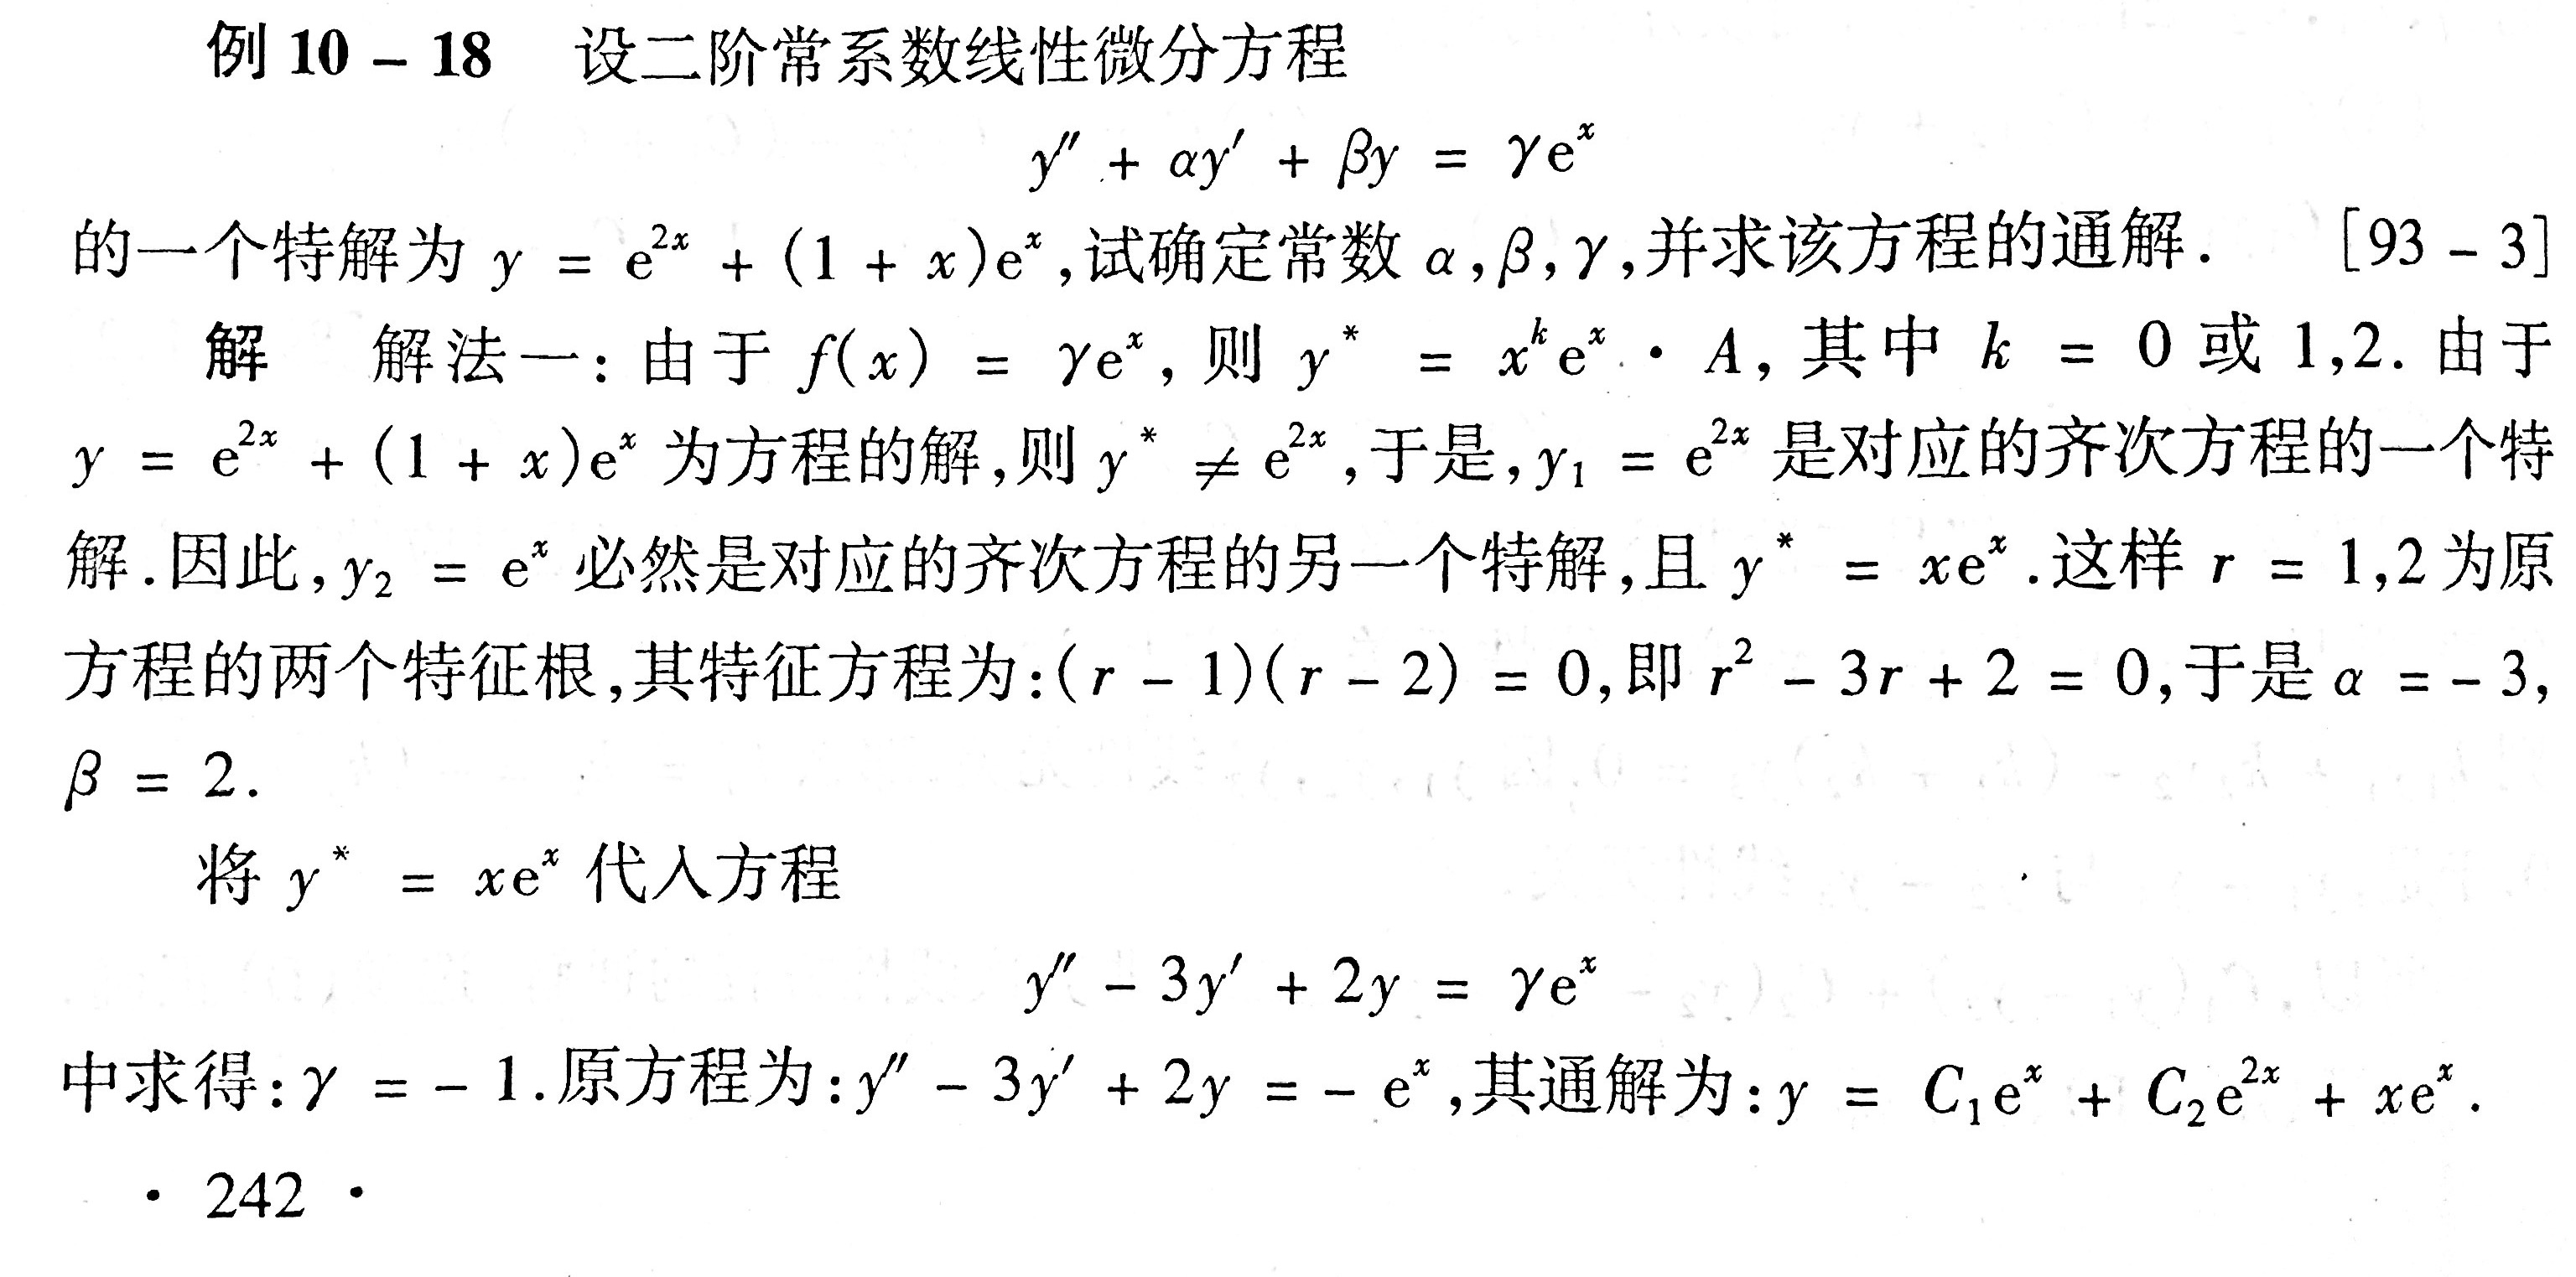
\includegraphics{./images/ch7/p242.jpg}}
\end{center}

{\it 这个解答没有问题,只是有些简略,导致不好理解。以下是我在此基础上进一步细化后的解答:}

{\bf 解:}由于右端函数为$\gamma e^x$,故原方程的特解应该形如
$$y^*=x^ke^x,$$
其中$k$可能为$0,1,2$。

根据线性微分方程解的结构定理,非齐次线性微分方程的特解可以由对应的齐次方程的多个特解与
该非齐次方程的一个特解相加得到。以下利用该结论进行分析:

注意到
$$(e^{2x})''+\alpha(e^{2x})'+\beta e^{2x}
=(4+2\alpha+\beta)e^{2x},$$
故$e^{2x}$不可能是原(非齐次)方程的特解,从而只能是对应的齐次方程的特解。
由此可知,$r=2$是方程的特征方程的根,

根据上一步的结论,可知$(1+x)e^x$中必然包含了原(非齐次)方程的特解,现在的问题是要将
这个特解的部分找出来。在此我们可以断言$(1+x)e^x$这个整体不可能就是原(非齐次)方程的特解
(因为它不具备前述$y^*$所应有的形式),特解只能是$e^x$和$xe^x$之一。
换言之,$e^x$和$xe^x$两者一个是原(非齐次)方程的特解,另一个是对应的齐次方程的特解。

若$xe^x$是对应的齐次方程的特解。根据二阶常系数齐次线性微分方程的通解公式,只有当$r=1$
为其特征方程的二重根时,解才会有形如$C_1e^x+C_2xe^x$的构造。而由前面的分析我们
已知$r=2$是特征方程的一个根,故$xe^x$只能是原(非齐次)方程的特解。进而$y=e^x$
必然是对应的齐次方程的特解。

综上可知,原(非齐次)方程有特解$xe^x$,其特征方程有相异实根$r=1,r=2$。

以下步骤和原解答相同,略。

\newpage

\section*{作业要求}

\begin{center}
	(试行版,2015年春季学期)
\end{center}

\begin{enumerate}
%   \setlength{\itemindent}{1cm}
  \item 作业内容分为基本题、上交题和思考题三部分,前两部分为必作题
  \item 上交与批改
  \begin{itemize}
    \item 作业分两部分分别上交
    \item 基础题每周上交一次,由本连负责人收齐交当周轮值的同学批改
    \item 上交题及思考题(选作)分三组,每周由其中一组上交,教员负责批改,
    每次上交须包括前两周未交过的部分
  \end{itemize}
  \item 基础题批改
  \begin{itemize}
    \item 按照事先排定的值班顺序,确保每人本学期至少轮值一次批改其他同学的作业
    \item 轮值同学批改其他同学作业后,须
    \begin{itemize}
      \item 根据作业正确率按百分制为其打分
      \item 在作业纸上签名
      \item 汇总作业情况交给本连负责人,汇总内容包括
      \begin{itemize}
        \item 每人的作业成绩
        \item 作业中大家错误或疑问较多的题目
      \end{itemize}
    \end{itemize}
    \item 连负责人将本连作业情况汇总后交总课代表
  \end{itemize}
\end{enumerate}

\newpage

{\bf 习题7.1-13}

\begin{center}
	\resizebox{!}{5cm}{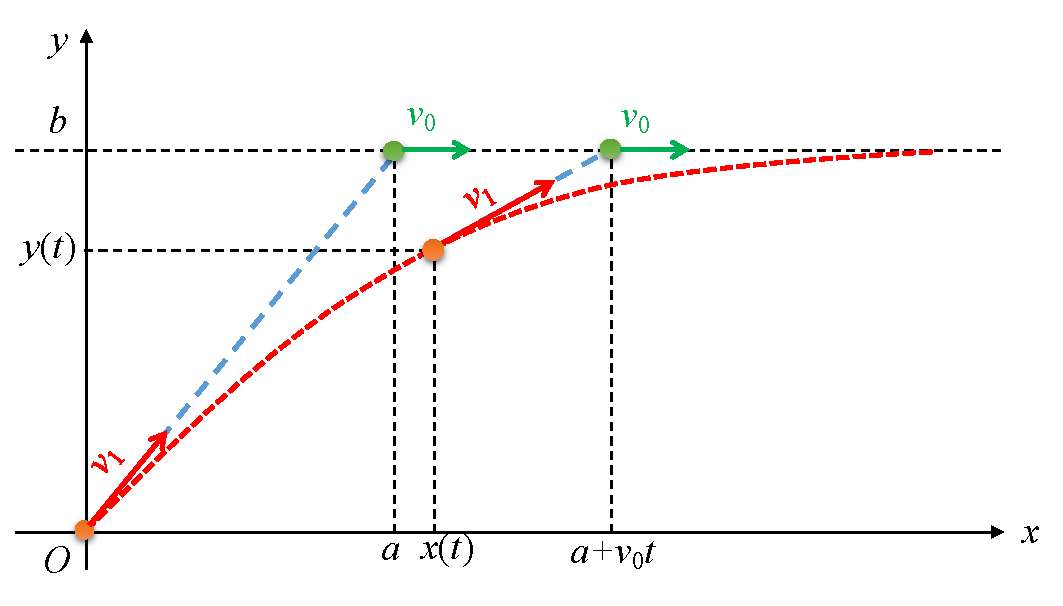
\includegraphics{./images/ch7/missile2Plane.pdf}}
\end{center}

如图:在$t$时刻,导弹走过的距离为
$$v_1t=\dint_0^x\sqrt{1+(y')^2}\d x\eqno{(1)},$$
又
$$y'=\df{b-y}{a+v_0t-x}\quad\Rightarrow\quad
t=\df1{v_0}\left(\df{b-y}{y'}+x-a\right),$$
带入(1)式,可得
$$\df{v_1}{v_0}\left(\df{b-y}{y'}+x-a\right)=\dint_0^x\sqrt{1+(y')^2}\d
x.$$
该式两边同时对$x$求导,整理后可得
$$\df{v_1}{v_0}(y-b)y''=(y')^2\sqrt{1+(y')^2}.$$
又由题意,显然有$y(0)=0,\;y'(0)=b/a$。综上,导弹的轨迹应满足如下的初值问题
$$
\left\{\begin{array}{l}
\df{v_1}{v_0}(y-b)y''=(y')^2\sqrt{1+(y')^2}\\
y'(0)=b/a\\
y(0)=0
\end{array}
\right.
$$